\documentclass[11pt,a4paper]{article}
\usepackage[utf8]{inputenc}
\usepackage[spanish]{babel}
\usepackage{hyperref}
\usepackage{graphicx}
\usepackage[table,xcdraw]{xcolor}
\usepackage{float}
\usepackage{lmodern,textcomp}
\usepackage{enumitem}
\usepackage[official]{eurosym}
\usepackage{listings}
\usepackage{xcolor}
\usepackage{filecontents}


\definecolor{javared}{rgb}{0.6,0,0} % for strings
\definecolor{javagreen}{rgb}{0.25,0.5,0.35} % comments
\definecolor{javapurple}{rgb}{0.5,0,0.35} % keywords
\definecolor{javadocblue}{rgb}{0.25,0.35,0.75} % javadoc
 
 
\lstset{language=Java,
basicstyle=\ttfamily,
keywordstyle=\color{javapurple}\bfseries,
stringstyle=\color{javared},
commentstyle=\color{javagreen},
morecomment=[s][\color{javadocblue}]{/**}{*/},
%numbers=left,
%numberstyle=\tiny\color{black},
%stepnumber=2,
%numbersep=10pt,
columns=fullflexible,
frame=single,
breaklines=true,
linewidth=13cm,
tabsize=4,
showspaces=false,
showstringspaces=false}

\author{Javier Ortuño Roig}
\title{Modelado y Diseño de Software}
\pagestyle{headings}

\begin{document}

\begin{titlepage}
\centering
{\bfseries\LARGE Universidad De Málaga \par}
\vspace{0.5cm}
{\scshape\Large Escuela Superior de Ingeniería Informática  \par}
\vspace{0.5cm}
{\scshape\Large Ingeniería de Software  \par}
\vspace{3cm}
{\scshape\Huge Práctica 4 \\ Patrones de Diseño \par}
\vspace{1.5cm}
{\scshape\Large Modelado y Diseño de Software \par}
\vspace{3cm}
{\Large \textbf{Grupo A3} \par}
{\Large Arjona Jiménez, Francisco de Paula \par}
{\Large Castillo Berná, David \par}
{\Large Ortuño Roig, Javier \par}
{\Large Ramet Espinosa, Alejandro \par}
{\Large Velasco López, Cristhian \par}
\vfill
{\Large \today \par}
\end{titlepage}

\tableofcontents

\newpage

\section{Ejercicio 1}
\subsection{Apartado a}

Java no dispone de mecanismos de exportación como tal, para la restricción de acceso de las diferentes clases a sus operaciones recurre a la visibilidad de los paquetes, (public, private, package, protected). Con esto una clase externa puede acceder tan solo a las operaciones públicas. La visibilidad protected indica que tan solo la misma clases y sus hijas pueden utilizarla y por último las operaciones private tan solo se pueden llamar en operaciones de la misma clase. 

	En eiffel al añadir ``feature'' podemos decir quienes podrán utilizar este método, con esto conseguimos una mayor simplicidad ya que al indicar directamente quienes pueden utilizarlo no tenemos que ir buscando si la clase exterior puede acceder o no a las operaciones de la clase inicial.



\subsection{Apartado b}

\subsubsection{Explicación textual}

El patrón que vamos a utilizar para resolver este ejercicio es el patrón estructural Proxy. Hemos utilizado este patrón ya que por propia definición se utiliza para el control de acceso al objeto principal. Es decir, la clase proxy indicará si una clase externa puede utilizar las operaciones de la clase principal o no. 
	
Al realizar esta implementación podremos observar que tenemos un total control de las clases, pero comparado con eiffel es más tedioso, ya que en eiffel con un comando controlamos todo, mientras que en java necesitamos una clase proxy que lo controle.

\subsubsection{Modelo}


\begin{figure}[H]
  \makebox[\textwidth][c]{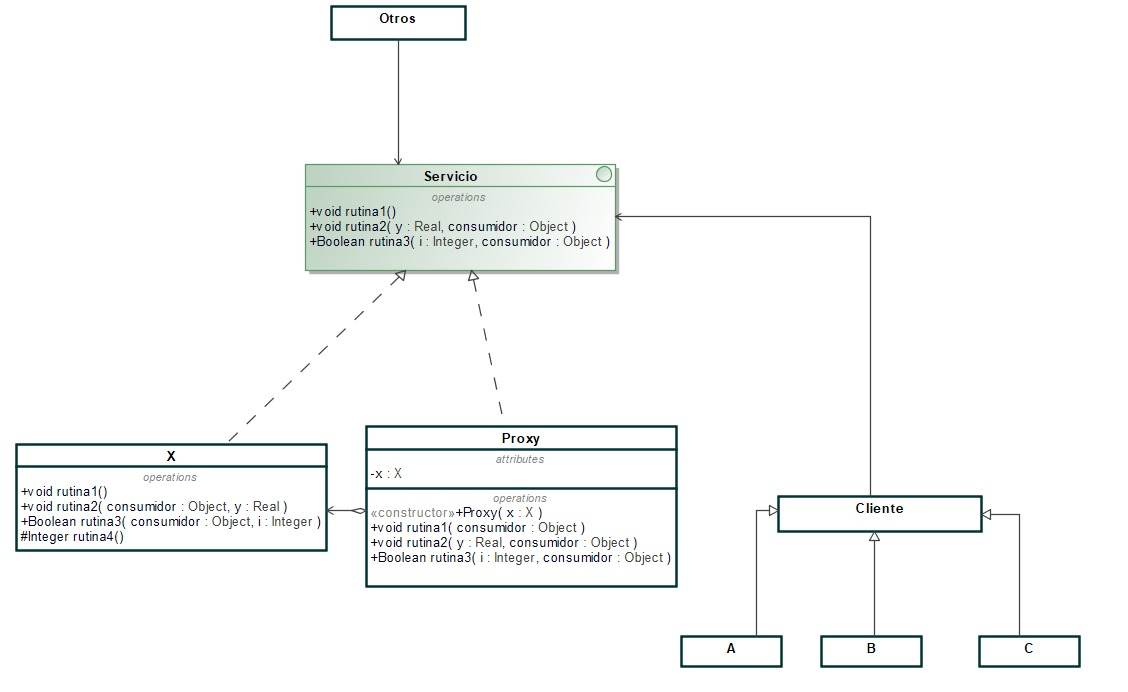
\includegraphics[width=1.4\textwidth]{images/modelo1.png}}%
\end{figure}



\subsubsection{Código}

Primero daremos una descripción y a continuación habrá imágenes con el código.

	Las clases A,B y C, son los tres tipos de clientes que pueden acceder a la clase X, que es la clase que realmente aporta los servicios. La clase Cliente tan solo sirve para indicar que las clases A, B y C son sus hijas para no tener código repetido.

	Como hemos indicado anteriormente a la clase Proxy le llega un cliente del tipo objeto, donde nosotros comprobamos de qué tipo es para saber si puede acceder a la operación de X que ha solicitado.
	
	Por último X y Proxy son hijas de la interfaz Servicio. En esta interfaz es la que indica que servicios aporta el proxy. La interfaz Servicio es un objeto imaginario, y la clase X es el objeto real, y el Proxy tiene la función de crear un objeto real si el cliente puede acceder a los servicios que solicita en la interfaz.


\lstinputlisting[language=Java, title=Interfaz: Servicio.Java]{images/src/Ejercicio1/Servicio.java}

\lstinputlisting[language=Java, title=Clase: X.Java]{images/src/Ejercicio1/X.java}

\lstinputlisting[language=Java, title=Clase: Proxy.Java]{images/src/Ejercicio1/Proxy.java}

\lstinputlisting[language=Java, title=Interfaz: Proxy.Java]{images/src/Ejercicio1/Cliente.java}

\lstinputlisting[language=Java, title=Clase: A.Java]{images/src/Ejercicio1/A.java}

\lstinputlisting[language=Java, title=Clase: B.Java]{images/src/Ejercicio1/B.java}

\lstinputlisting[language=Java, title=Clase: C.Java]{images/src/Ejercicio1/C.java}


\section{Ejercicio 2}
\subsection{Apartado a}

\subsubsection{Explicación textual}

En este apartado vamos a utilizar el patrón de diseño ``Estado''. Esto se debe a nuestra necesidad de querer alterar el comportamiento de la clase ``Biestable'' según el estado en el que se encuentre.

Concretamente, deseamos dos estados para el mismo, ``Rojo'' y ``Verde''. Ambos se implementarán como subclases de una clase abstracta ``Estado'', que contendrá los métodos propios de la clase ``Biestable'', pues queremos que según el estado en el que se encuentre, actúe de una manera u otra.

Por lo tanto, nuestra clase ``Biestable'' contendrá una instancia de ``Estado'', que podrá ser o ``Rojo'' o ``Verde''.

En cuanto a los métodos del biestable:

\begin{itemize}
\item abrir():

	\begin{itemize}
	\item Estado ``Rojo'': permitirá a un ``Biestable'' pasar de un estado ``Rojo'' a ``Verde''.
	\item Estado ``Verde'': devolverá un mensaje de error.
	\end{itemize}
	
\item cerrar():

	\begin{itemize}
	\item Estado ``Rojo'': devolverá un mensaje de error.
	\item Estado ``Verde'':  permitirá a un ``Biestable'' pasar de un estado ``Verde'' a ``Rojo''.

	\end{itemize}
	
\item estado() : devolverá un string correspondiente al estado en el que me encuentro.
\end{itemize}

Adicionalmente, hemos utilizado el patrón “Singleton” para reutilizar las instancias de los estados, ya que en otro caso, con la llamada a los métodos, estaríamos creando constantemente nuevos estados.

Para aplicarlo, la clase contendrá un atributo estático correspondiente a una instancia de la misma clase. Por otro lado, encontramos un método getInstance(), que nos permitirá crear esta instancia estática si no se ha creado anteriormente (a través del constructor privado de la clase), o bien devolver dicha instancia ya creada.


\subsubsection{Modelo}

\begin{figure}[H]
  \makebox[\textwidth][c]{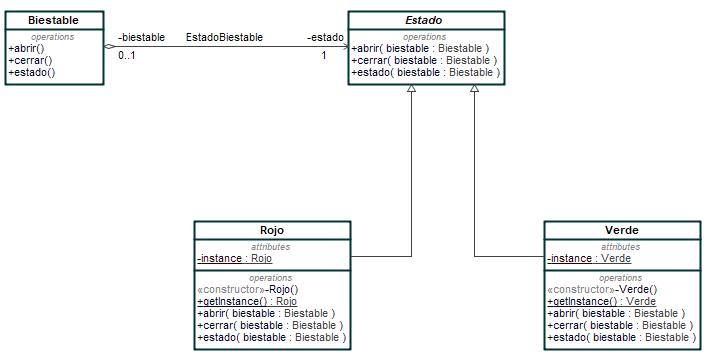
\includegraphics[width=1.4\textwidth]{images/modelo2.png}}%
\end{figure}


\subsubsection{Pseudocódigo}

Dado que el pseudocódigo es muy parecido al código en Java se dejará solo el código para no sobrecargar la memoria con información repetida.

\subsubsection{Código}

\lstinputlisting[language=Java, title=Clase: Biestable.Java]{images/src/Ejercicio2/a/Biestable.java}

\lstinputlisting[language=Java, title=Clase abstracta: Estado.Java]{images/src/Ejercicio2/a/Estado.java}

\lstinputlisting[language=Java, title=Clase: Rojo.Java]{images/src/Ejercicio2/a/Rojo.java}

\lstinputlisting[language=Java, title=Clase: Verde.Java]{images/src/Ejercicio2/a/Verde.java}

\subsection{Apartado b}

\subsubsection{Explicación textual}

Al igual que en el apartado anterior, utilizaremos el patrón de diseño ``Estado'' para implementar la clase ``Triestable'', añadiendo esta vez una nueva subclase ``Amarillo'', que será un estado intermedio entre ``Rojo'' y ``Verde''.

Como queremos que en nuestro sistema haya tanto biestables como triestables, ambos tendrán un atributo ``Estado''. Sin embargo, debido a que un biestable no puede estar en un estado ``Amarillo'', hemos añadido una restricción OCL para evitar esto:

\begin{itemize}
\item \emph{not self.estado.oclIsTypeOf(Amarillo):} En el contexto de un Biestable, su estado no podrá ser del tipo ``Amarillo''
\end{itemize}


En cuanto a los métodos del triestable:

\begin{itemize}
\item abrir():

	\begin{itemize}
	\item Estado ``Rojo'': permitirá a un ``Biestable'' pasar de un estado ``Rojo'' a ``Amarillo''.
	\item Estado ``Amarillo'' : permitirá a un ``Biestable'' pasar de un estado ``Amarillo'' a ``Verde''.

	\item Estado ``Verde'': devolverá un mensaje de error.
	\end{itemize}
	
\item cerrar():

	\begin{itemize}
	\item Estado ``Rojo'': devolverá un mensaje de error.
	\item Estado ``Amarillo'' : permitirá a un ``Biestable'' pasar de un estado ``Amarillo'' a ``Rojo''.
	\item Estado ``Verde'':  permitirá a un ``Biestable'' pasar de un estado ``Verde'' a ``Amarillo''.

	\end{itemize}
	
\item estado() : devuelve una cadena string que muestra el estado en el que se encuentra el triestable.
\end{itemize}


Adicionalmente, hemos utilizado el patrón “Singleton” para reutilizar las instancias de los estados, ya que en otro caso, con la llamada a los métodos, estaríamos creando constantemente nuevos estados.

Para aplicarlo, la clase contendrá un atributo estático correspondiente a una instancia de la misma clase. Por otro lado, encontramos un método getInstance(), que nos permitirá crear esta instancia estática si no se ha creado anteriormente (a través del constructor privado de la clase), o bien devolver dicha instancia ya creada.



\subsubsection{Modelo}

\begin{figure}[H]
  \makebox[\textwidth][c]{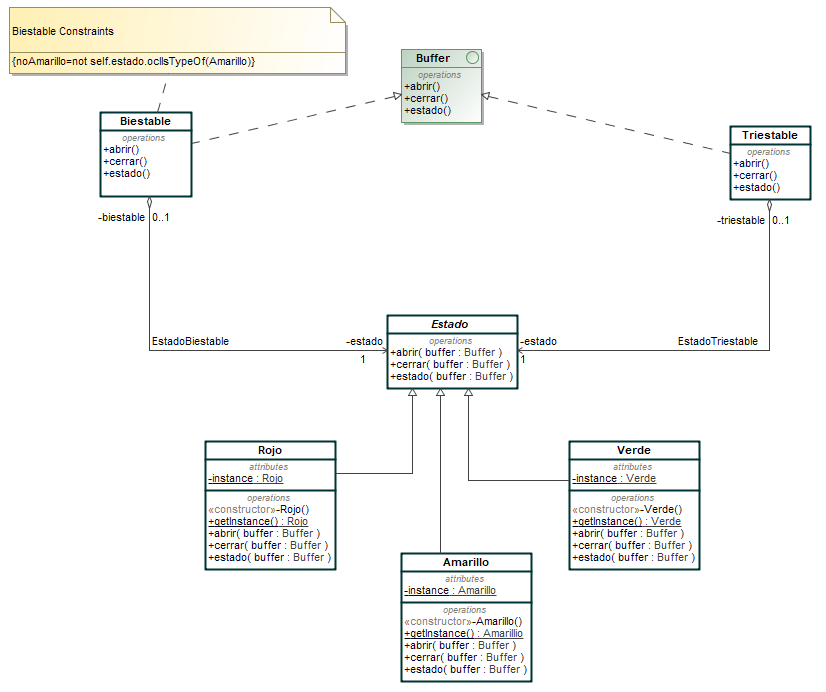
\includegraphics[width=1.4\textwidth]{images/modelo3.png}}%
\end{figure}

\subsubsection{Pseudocódigo}

Dado que el pseudocódigo es muy parecido al código en Java se dejará solo el código para no sobrecargar la memoria con información repetida.


\subsubsection{Código}

\lstinputlisting[language=Java, title=Interfaz: Buffer.Java]{images/src/Ejercicio2/b/Buffer.java}

\lstinputlisting[language=Java, title=Clase: Biestable.Java]{images/src/Ejercicio2/b/Biestable.java}

\lstinputlisting[language=Java, title=Clase: Triestable.Java]{images/src/Ejercicio2/b/Triestable.java}

\lstinputlisting[language=Java, title=Clase abstracta: Estado.Java]{images/src/Ejercicio2/b/Estado.java}

\lstinputlisting[language=Java, title=Clase: Rojo.Java]{images/src/Ejercicio2/b/Rojo.java}

\lstinputlisting[language=Java, title=Clase: Amarillo.Java]{images/src/Ejercicio2/b/Amarillo.java}

\lstinputlisting[language=Java, title=Clase: Verde.Java]{images/src/Ejercicio2/b/Verde.java}

\subsection{Apartado c}

\subsubsection{Explicación textual}
Al igual que en el apartado anterior, utilizaremos el patrón de diseño ``Estado'' para implementar las clases ``Biestable'' y ``Triestable''.

\vspace{0.25cm}

En este caso, para implementar el cambio de ``Biestable'' a ``Triestable'', utilizaremos el patrón de diseño ``Decorador''. Con esto conseguiremos añadir la funcionalidad de la clase ``Triestable'' a nuestra clase ``Biestable''.

\vspace{0.25cm}

Para ello el ``Biestable'' contendrá un objeto que implementará la interfaz ``Buffer'', inicialmente a null. 

\vspace{0.25cm}

Este objeto se inicializará a un objeto de tipo ``Triestable'' tras la llamada al método cambio() del ``Biestable''. De esta manera, cuando se vuelvan a invocar a los métodos abrir(), cerrar() y estado(), serán los métodos del buffer (Triestable) los que se ejecuten, actuando el ``Biestable'' como un ``Triestable''.

\vspace{0.25cm}

Adicionalmente, hemos utilizado el patrón “Singleton” para reutilizar las instancias de los estados, ya que en otro caso, con la llamada a los métodos, estaríamos creando constantemente nuevos estados.

\vspace{0.25cm}

Para aplicarlo, la clase contendrá un atributo estático correspondiente a una instancia de la misma clase. Por otro lado, encontramos un método getInstance(), que nos permitirá crear esta instancia estática si no se ha creado anteriormente (a través del constructor privado de la clase), o bien devolver dicha instancia ya creada.



\subsubsection{Modelo}


\begin{figure}[H]
  \makebox[\textwidth][c]{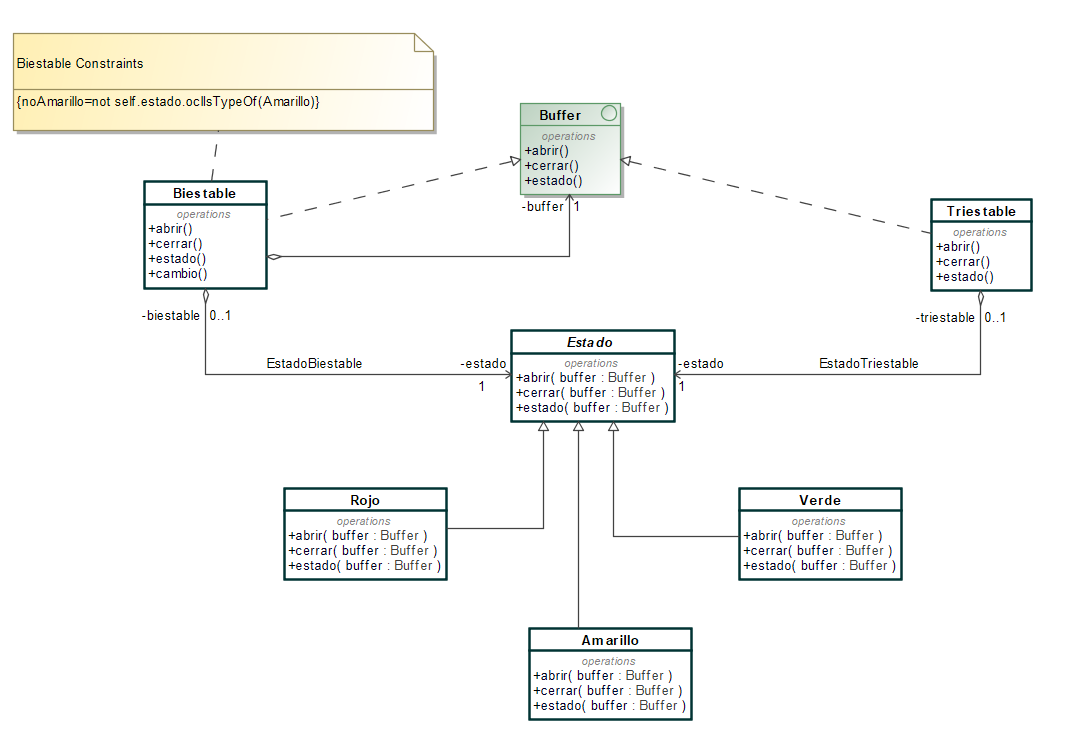
\includegraphics[width=1.4\textwidth]{images/modelo4.png}}%
\end{figure}

\subsubsection{Pseudocódigo}

Dado que el pseudocódigo es muy parecido al código en Java se dejará solo el código para no sobrecargar la memoria con información repetida.

\subsubsection{Código}

\lstinputlisting[language=Java, title=Interfaz: Buffer.Java]{images/src/Ejercicio2/c/Buffer.java}

\lstinputlisting[language=Java, title=Clase: Biestable.Java]{images/src/Ejercicio2/c/Biestable.java}

\lstinputlisting[language=Java, title=Clase: Triestable.Java]{images/src/Ejercicio2/c/Triestable.java}

\lstinputlisting[language=Java, title=Clase abstracta: Estado.Java]{images/src/Ejercicio2/c/Estado.java}

\lstinputlisting[language=Java, title=Clase: Rojo.Java]{images/src/Ejercicio2/c/Rojo.java}

\lstinputlisting[language=Java, title=Clase: Amarillo.Java]{images/src/Ejercicio2/c/Amarillo.java}

\lstinputlisting[language=Java, title=Clase: Verde.Java]{images/src/Ejercicio2/c/Verde.java}


\section{Ejercicio 3}


\subsection{Explicación textual}

En este ejercicio hemos usado el patrón estrategia porque nos requería diferenciar el algoritmo según diferentes criterios, permitiendo así definir una familia de algoritmos, encapsulandolos en clases distintas y haciéndolos intercambiables a su vez. Para desarrollarlo hemos creado la interfaz ‘Ordenación', la cual implementan las subclases 'OrdenacionFrom', 'OrdenacionSubject', 'OrdenacionPriority' y  'OrdenacionDate', que tal y como su nombre indica cada subclase hace referencia a su propio algoritmo del método 'before()', definiendo así una clase estrategia por cada uno de ellos.


\subsection{Modelo}

\begin{figure}[H]
  \makebox[\textwidth][c]{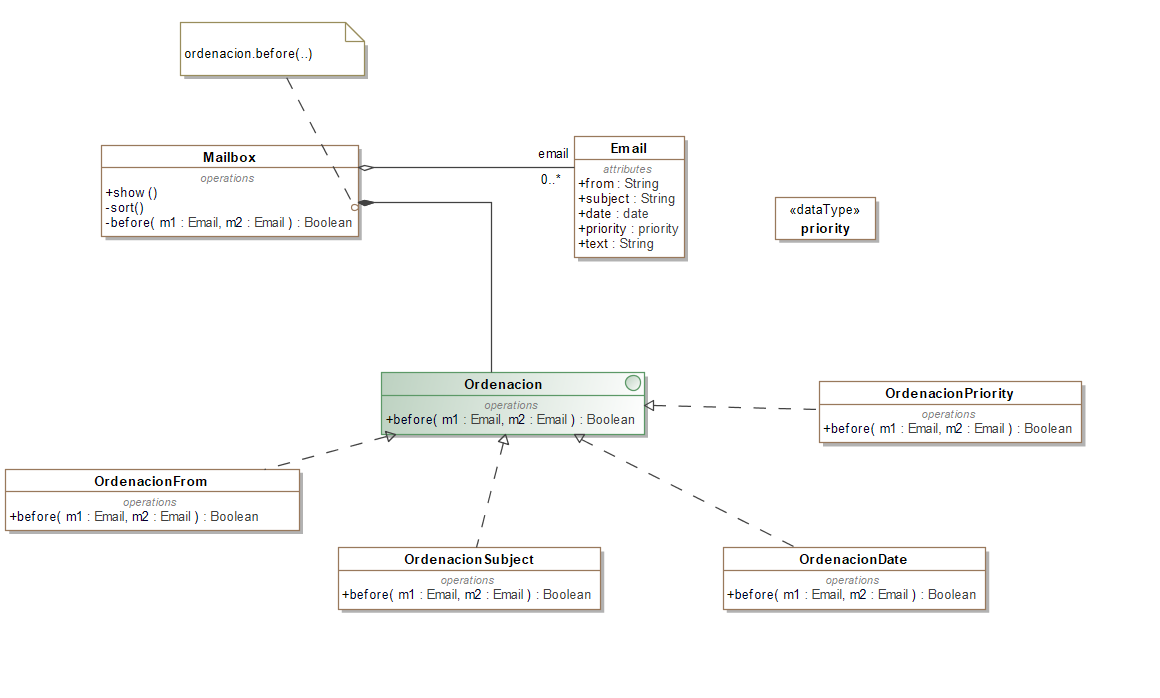
\includegraphics[width=1.4\textwidth]{images/modelo5.png}}%
\end{figure}

\subsection{Código}

\lstinputlisting[language=Java, title=Clase: Email.Java]{images/src/Ejercicio3/Email.java}

\lstinputlisting[language=Java, title=Clase: Mailbox.Java]{images/src/Ejercicio3/Mailbox.java}

\lstinputlisting[language=Java, title=Interfaz: Ordenacion.Java]{images/src/Ejercicio3/Ordenacion.java}

\lstinputlisting[language=Java, title=Clase: OrdenacionDate.Java]{images/src/Ejercicio3/OrdenacionDate.java}

\lstinputlisting[language=Java, title=Clase: OrdenacionFrom.Java]{images/src/Ejercicio3/OrdenacionFrom.java}

\lstinputlisting[language=Java, title=Clase: OrdenacionPriority.Java]{images/src/Ejercicio3/OrdenacionPriority.java}

\lstinputlisting[language=Java, title=Clase: OrdenacionSubject.Java]{images/src/Ejercicio3/OrdenacionSubject.java}

\lstinputlisting[language=Java, title=Clase: Priority.Java]{images/src/Ejercicio3/Priority.java}



\section{Patrones de diseño usados}

Proxy: \url{(https://refactoring.guru/es/design-patterns/proxy)}

State: \url{(https://refactoring.guru/es/design-patterns/state)}

Singleton: \url{(https://refactoring.guru/es/design-patterns/singleton)}

Strategy: \url{(https://refactoring.guru/es/design-patterns/strategy)}


\end{document}
